\section{Definice ovládání, řízení a regulace(řízení bez a se zpětnou vazbou),výhody a nevýhody.Základní veličiny a přenosy. Rozdělení řízení podle různých kritérií. PID regulátory, základní složky a vlastnosti. Statická analýza zpětnovazebních obvodů. Standartní přenosy ve zpětnovazebním řízení, charakteristický polynom. Věta o počáteční a konečné hodnotě, požadavky na ustálené hodnoty.}
\subsection*{Řízení}
Cílevědomé působení na řízený objekt, s cílem dosáhnout požadovaných výsledků. Dělí se na ovládání a regulaci.

\subsection*{Ovládání}
tj. bez zpětné vazby\\
bez znalosti skutečné hodnoty na výstupu, tím pádem nelze kompenzovat vliv poruchových signálů, nelze zajistit správné sledování v případě změn parametrů soustavy\\

\subsection*{Regulace}
Krom regulační odchylky je zde i regulátor, který generuje akční zásah na základě odchylky a poruchy.
\begin{figure}[H]
    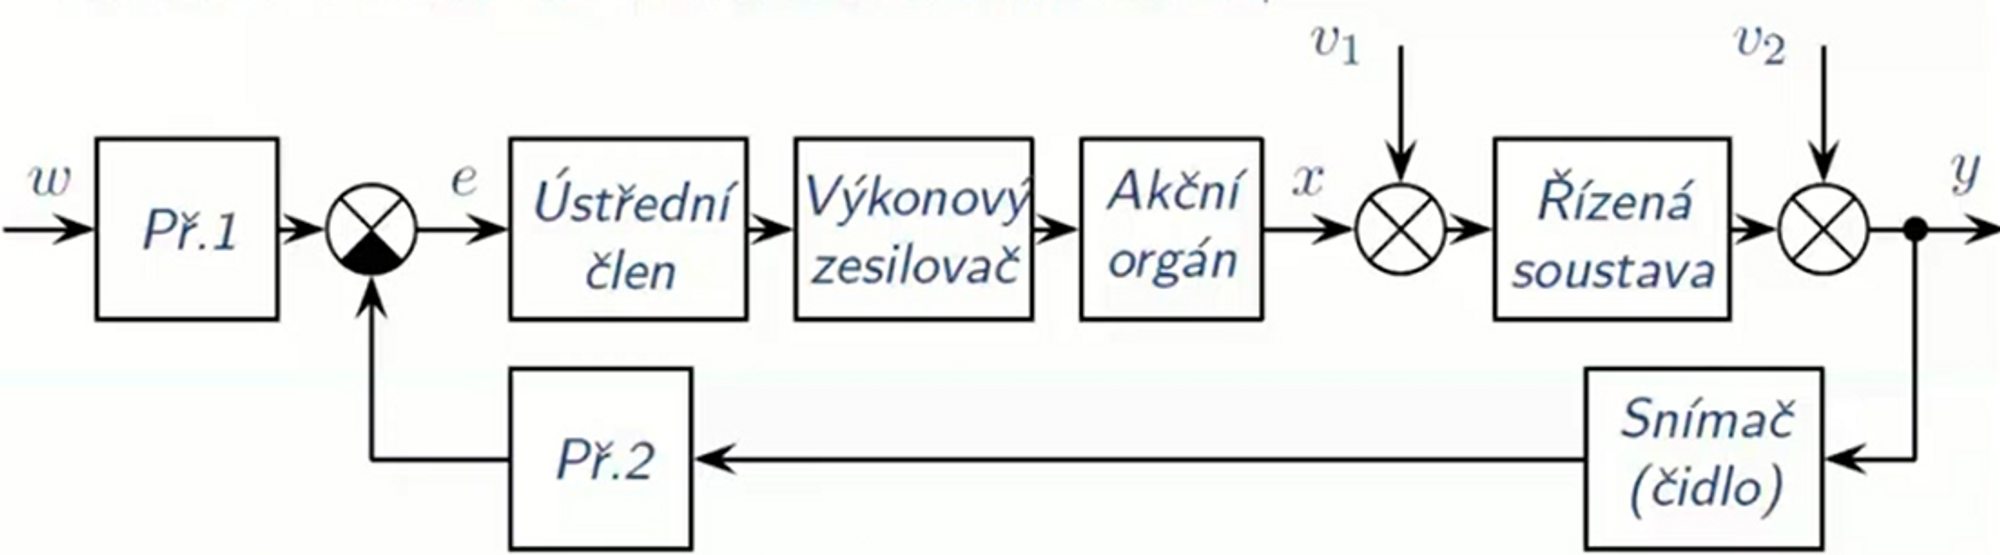
\includegraphics[scale = 0.45]{images/reg.soustava.png}
    \caption{Rozšířená regulačnní smyčka}
\end{figure}
\subsection*{Základní veličiny a přenosy}
\begin{figure}[H]
    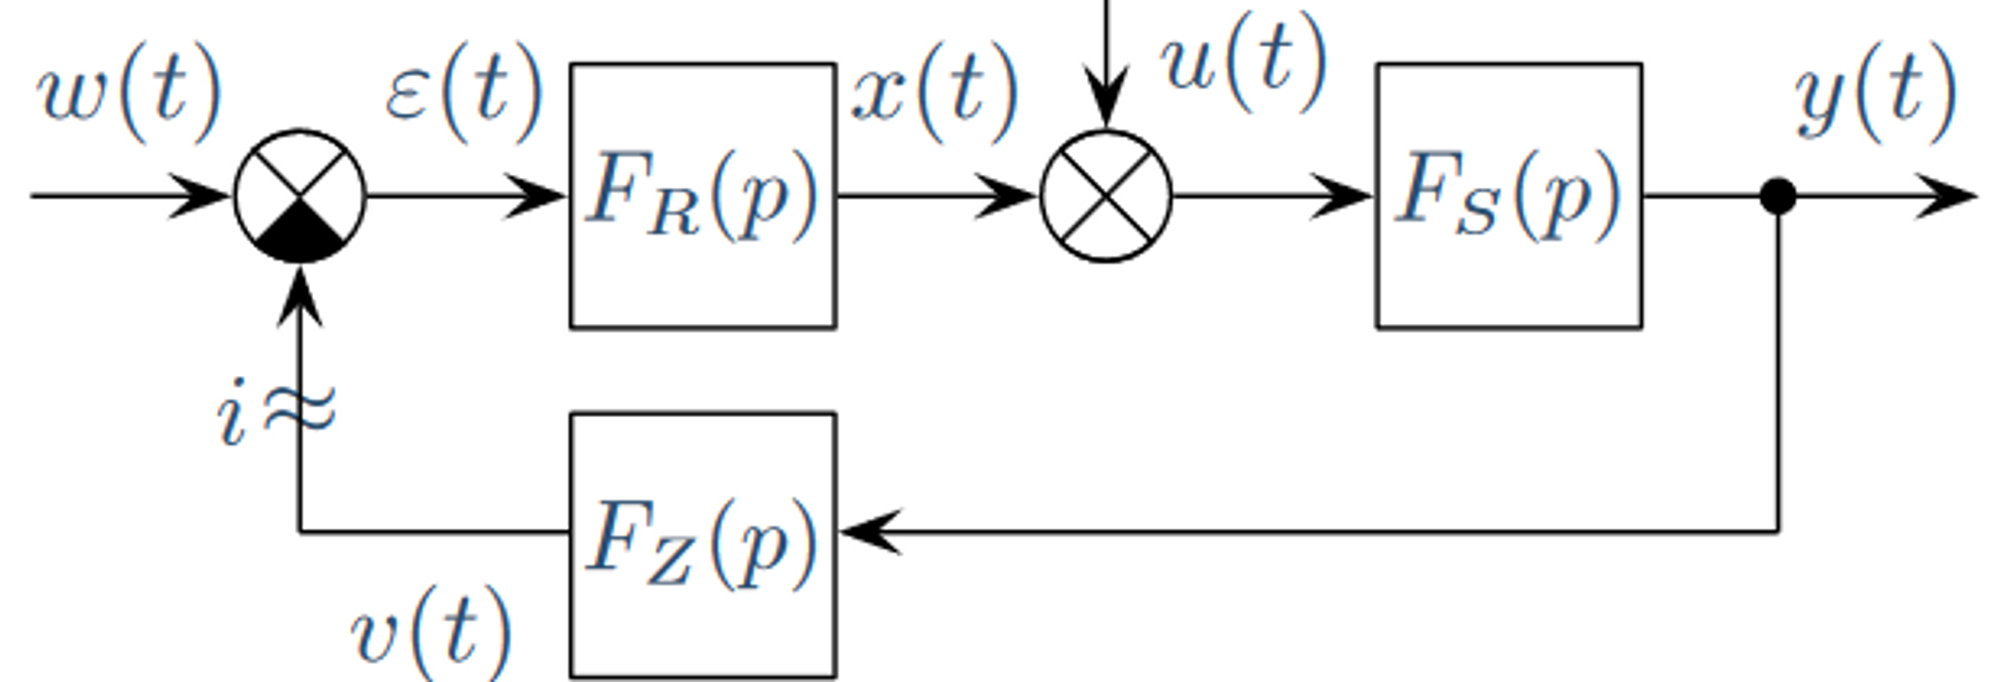
\includegraphics[scale = 0.45]{images/reg.soustava2.png}
    \caption{Regulačnní smyčka}
\end{figure}
w(t) \dots vstupní signál \\
$\varepsilon(t)$ \dots odchylka \\
x(t) \dots akční veličina \\
u(t) \dots porucha \\
y(t) \dots výstupní signál\\
v(t) \dots výstup ze zpětné vazby\\
i    \dots výstup f0 za předpokladu, že je zpětná vazba rozpojená\\

\noindent
Přenos regulované soustavy:
\begin{equation}
    F_S(p) = \frac{Y(p)}{X(p)}
\end{equation}
Přenos regulátoru:
\begin{equation}
    F_R(p) = \frac{X(p)}{\varepsilon(p)}
\end{equation}
Přenos zpětné vazby:
\begin{equation}
    F_Z(p) = \frac{V(p)}{Y(p)}
\end{equation}
Otevřené smyčky:
\begin{equation}
    F_0(p) = \frac{V(p)}{\varepsilon(p)}
\end{equation}
Přenos řízení:
\begin{equation}
    F_W(p) = \frac{Y(p)}{W(p)}
\end{equation}
Přenos poruchy:
\begin{equation}
    F_U(p) = \frac{Y(p)}{U(p)}
\end{equation}
Přenos odchylky:
\begin{equation}
    F_E(p)=\frac{E(p)}{W(p)}
\end{equation}
Přenos akční veličiny:
\begin{equation}
    F_a(p) = \frac{X(p)}{W(p)}
\end{equation}
\subsection*{Rozdělení řízení podle kritérií}
Řízení na konstantní hodnotu:
\begin{itemize}
    \item obecně regulátory
    \item Žádaná hodnota se s časem němění
    \item Úkolem je pouze kompenzace poruch, které na systém působí.
    \item např. frekvence, napětí, hladina vody, teplota
\end{itemize}
Řízení hodnoty s neznámým průběhem
\begin{itemize}
    \item cíl zajistit co nejpřesnější a nejpřesnější sledování průběhu - obecně servomechanismus
    \item Úloha kompenzace poruch je druhotná, primární je zajištění co nejrychlejší a nejvěrnější shdoy řícící a řízené veličiny
    \item sledování polohy
\end{itemize}
Řízení na hodnoty s předem známým průběhem:
\begin{itemize}
    \item sledování výstupu a kompenzace poruch jsou rovnocenné
    \item lze použít řídící algoritmus - programově řízené
\end{itemize}
\subsection*{PID regulátor}
Obsahuje proporciální, integrační a derivační složku
\begin{equation}
    F_R(p) = r_0 + \frac{r_i}{p} + r_d p= K_R(1+T_Dp+\frac{1}{T_Ip}) = k_r\frac{(T_1p+1)(T_2p+1)}{p}
\end{equation}
proporciální složka == offset, větší zesílení, větší přesnost \\
integrační složka - zhoršuje dynamické vlastnosti, zpomaluje regulační děj, slouží k nulové ustálené odchylce nebo poruše\\
derivační složka - zlepšuje dynamické vlastnosti, zrychluje regulační děj, zesiluje působení šumu\\
Pásmo proporcionality - udává, jaká je nutná změna ke změně výstupní veličiny regulátoru
\begin{equation}
    pp = \frac{1}{r_0}
\end{equation}
\begin{figure}[H]
    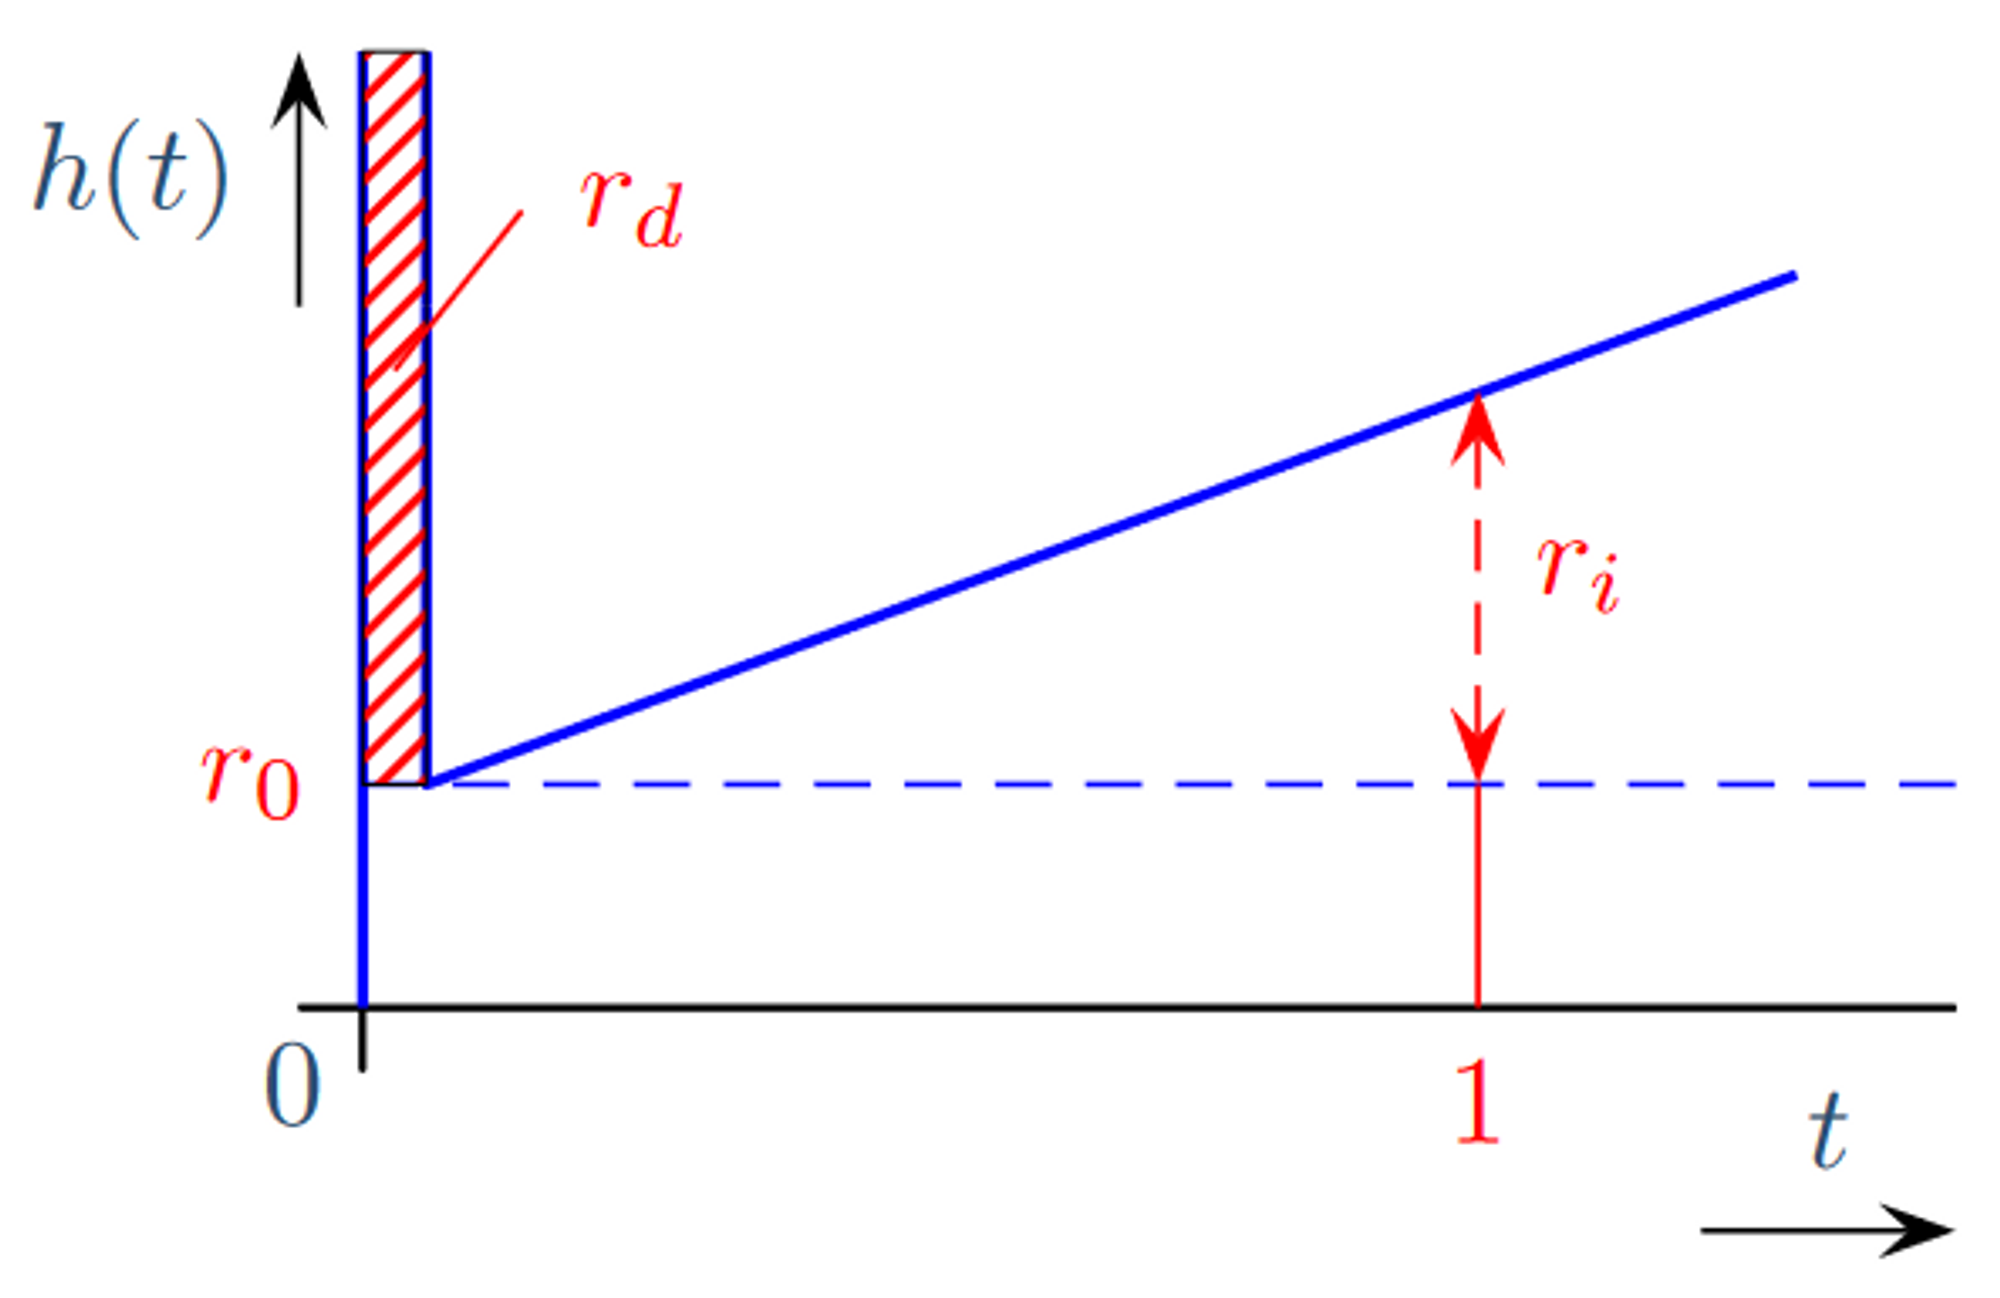
\includegraphics[scale = 0.3]{images/pasmo_proporcionality.png}
    \caption{PID}
\end{figure}
Rozdíl mezi reálným PID a PID:
\begin{itemize}
    \item reálný má realizační konstantu ve jmenovateli
    \item křivky jsou více zaoblené(viz obr. č. \ref{PID})
\end{itemize}
Reálný PID je pak, kde \(\varepsilon << T_1,T_2\):
\begin{equation}
    F_R(p) = \frac{X(p)}{E(p)} = K_R\frac{(T_1p + 1)(T_2p+1)}{p(\varepsilon p +1)}
\end{equation}
\begin{figure}[H]
    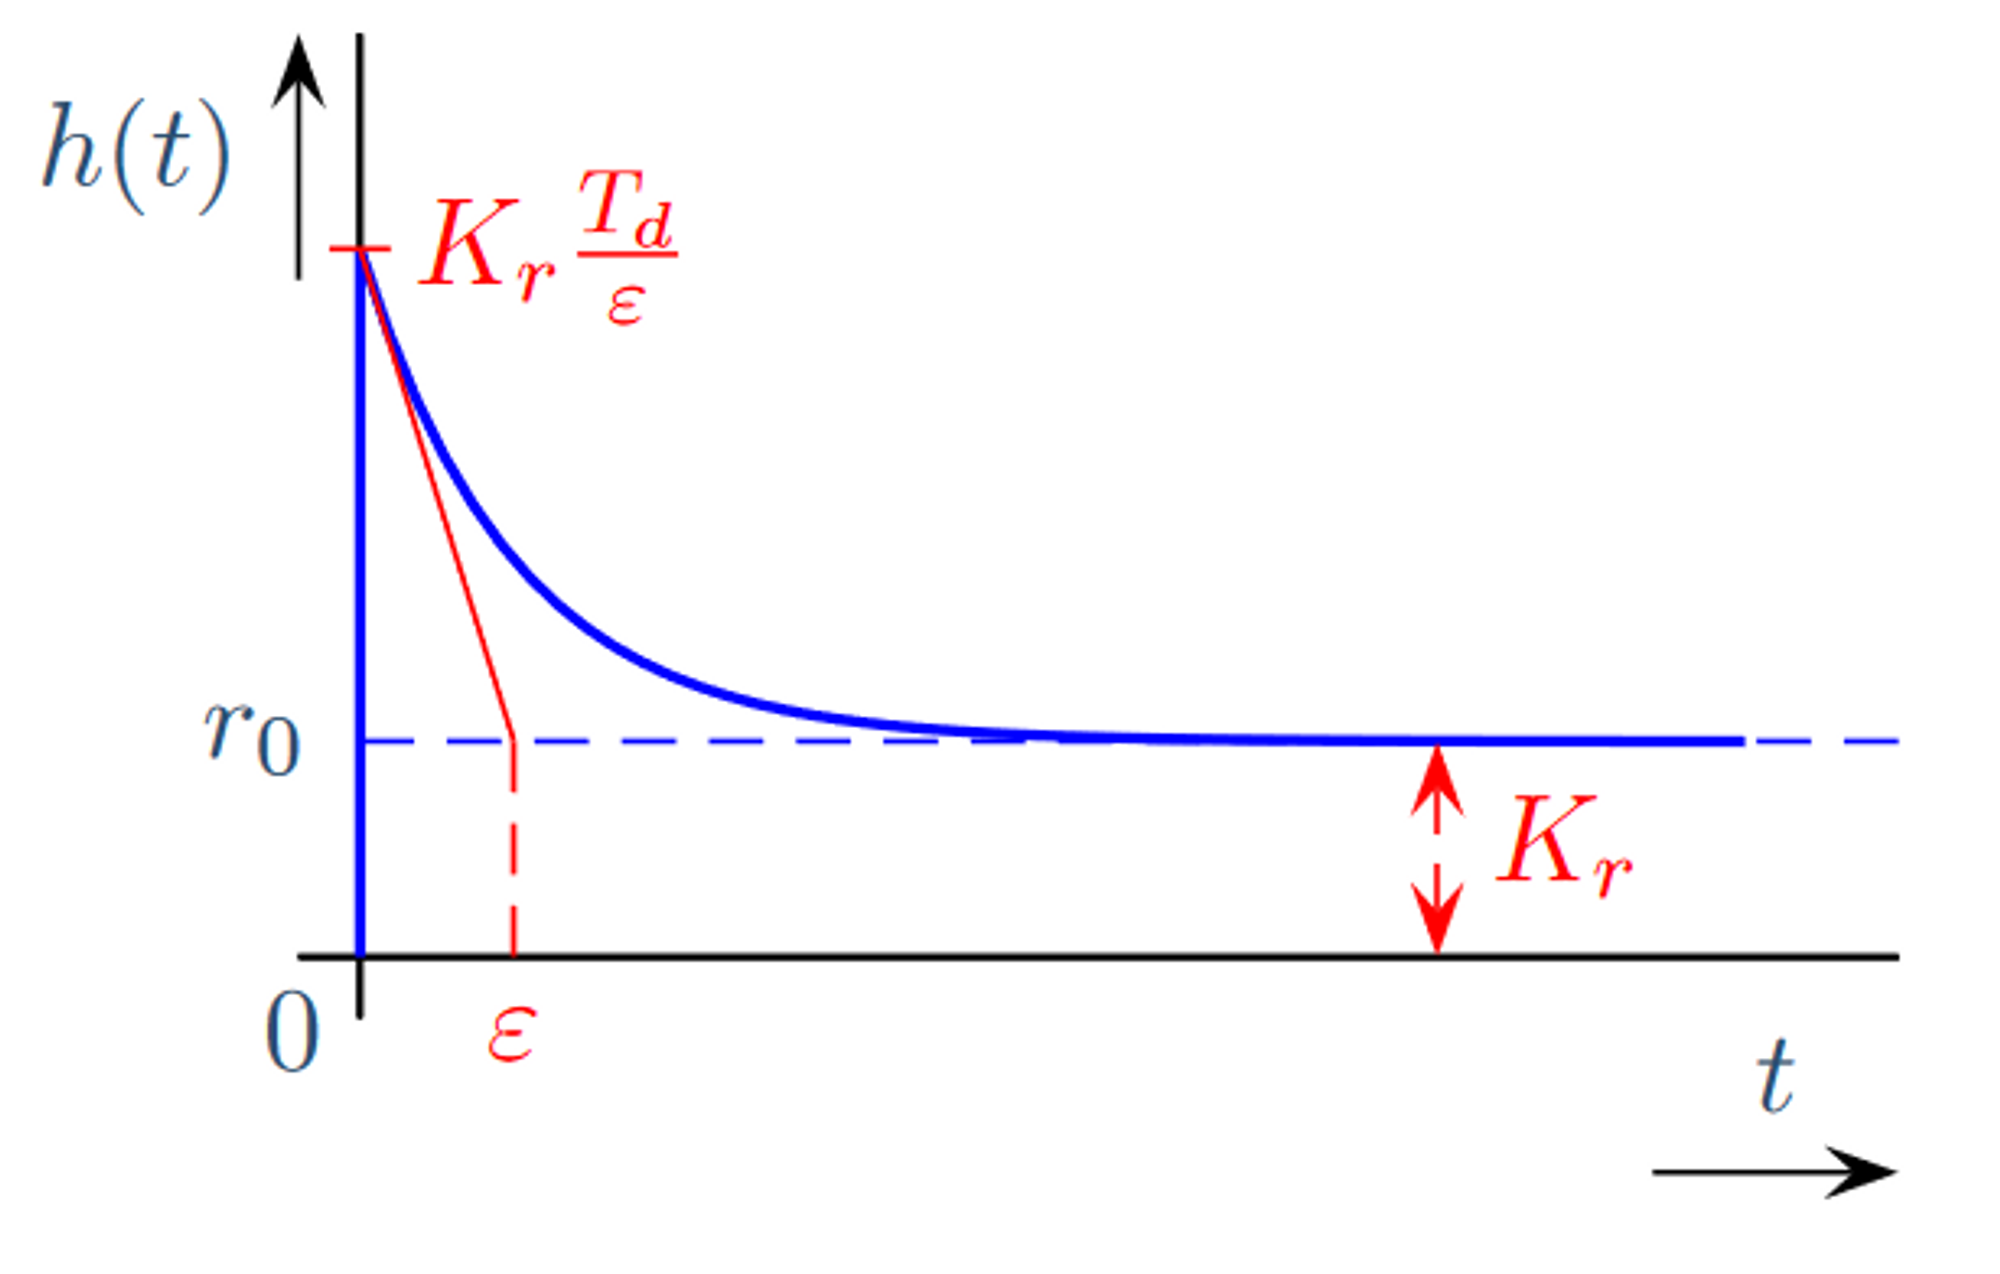
\includegraphics[scale = 1]{images/PID.png}
    \caption{Reálný PID}
    \label{PID}
\end{figure}
\subsection*{Statická analýza zpětnovazebních obvodů}
Přetlumené soustavy
\begin{itemize}
    \item bez kmitání
    \item sériové spojení setrvačných článků - všechny póly reálné a záporné
\end{itemize}
\begin{equation}
    F(p) =\frac{K}{(Tp+1)^n}
\end{equation}
\begin{figure}[H]
    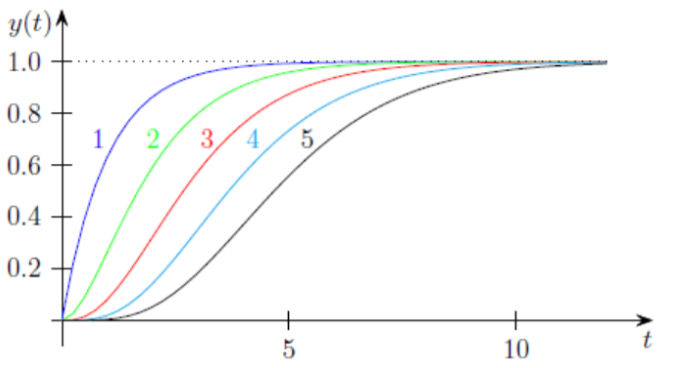
\includegraphics[scale = 1]{images/tlumeni.png}
    \caption{regulační křivky s rozdílným n}
\end{figure}

Kmitavé soustavy:
\begin{itemize}
    \item v přenosové funkci se vyskytují komplexně sdružené póly
    \item v časových odezvách (impulzní a přechodová charakteristika) se nacházejí harmonické funkce sin a cos
    \item pokud kmitavé póly nejsou dominantní, kmitání nemusí být patrné
\end{itemize}
\begin{equation}
    F(p) = \frac{k}{(p^2+p+1)(0,1p+1)}
\end{equation}

Soustavy s astatismem:
\begin{itemize}
    \item přítomnost nezavazbeného integrátoru
    \item obsahují pól v počátku
    \item náchylné k nestabilitě
    \item přechodovka odchází do nekonečna
    \item zhoršuje vlastnosti řízení, ale nulová ustálená odchylka
\end{itemize}

Soustavy s neminimální fází:
\begin{itemize}
    \item jedna nebo více nul v pravé polorovině
    \item chová se divně, nastává podkmit u jednotkového skoku na začátku. Přejde do záporných hodnot, ale pak se vrátí. Například když do kamen nasypeme uhelný prach, prvně se oheň zadusí, ale chytne a dojde ke zvýšení teploty.
    \item ve frekvenčních charakteristikách neplatí vztah mezi sklonem a fází frekvenční charakteristiky
\end{itemize}

Soustavy s dopravním zpožděním:
\begin{itemize}
    \item $y(t) = x(t-d)$ v obraze $F(p) = e^{-dp}$
\end{itemize}
\newpage

\subsection*{Charakteristický polynom}
\begin{equation}
    1+F_0(p)
\end{equation}
Všechny přenosy uzavřeného obvodu mají ve jmenovateli tento tvar\\
když jsou jeho reálné části kořenů menší nule, je stabilní, pokud jsou rovny nule, tak je na mezi stability\\
\subsection*{Věta o počáteční a konečné hodnotě, požadavky na ustálené hodnoty}
\begin{figure}[H]
    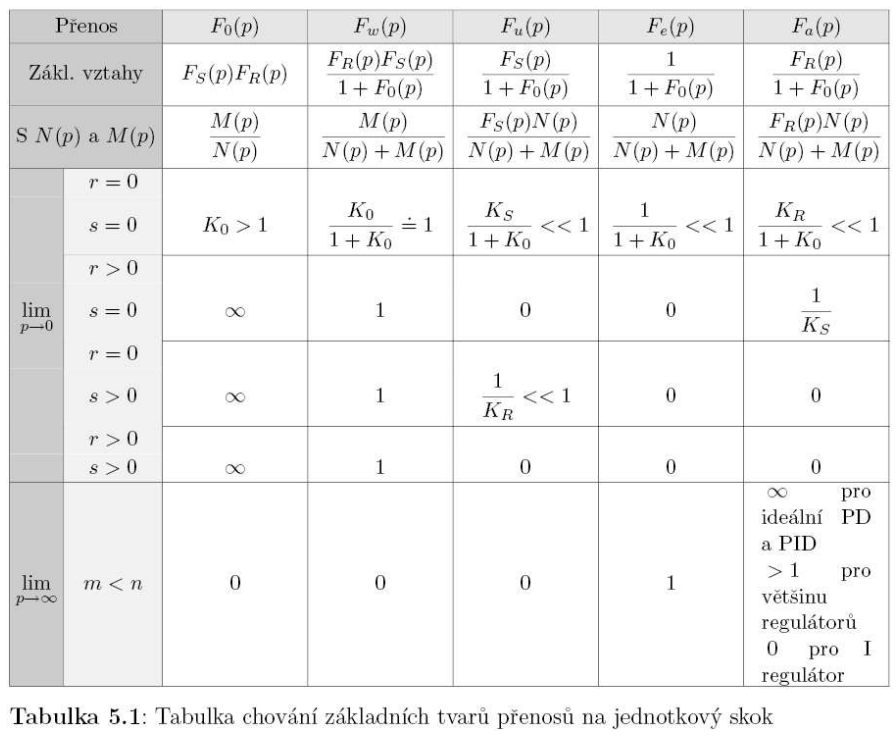
\includegraphics[scale = 0.8]{images/tvary_prenosu.png}
\end{figure}
Ustálená odchylka pro různé vstupy a počet integrátorů v soustavě a regulátoru:
\begin{figure}[H]
    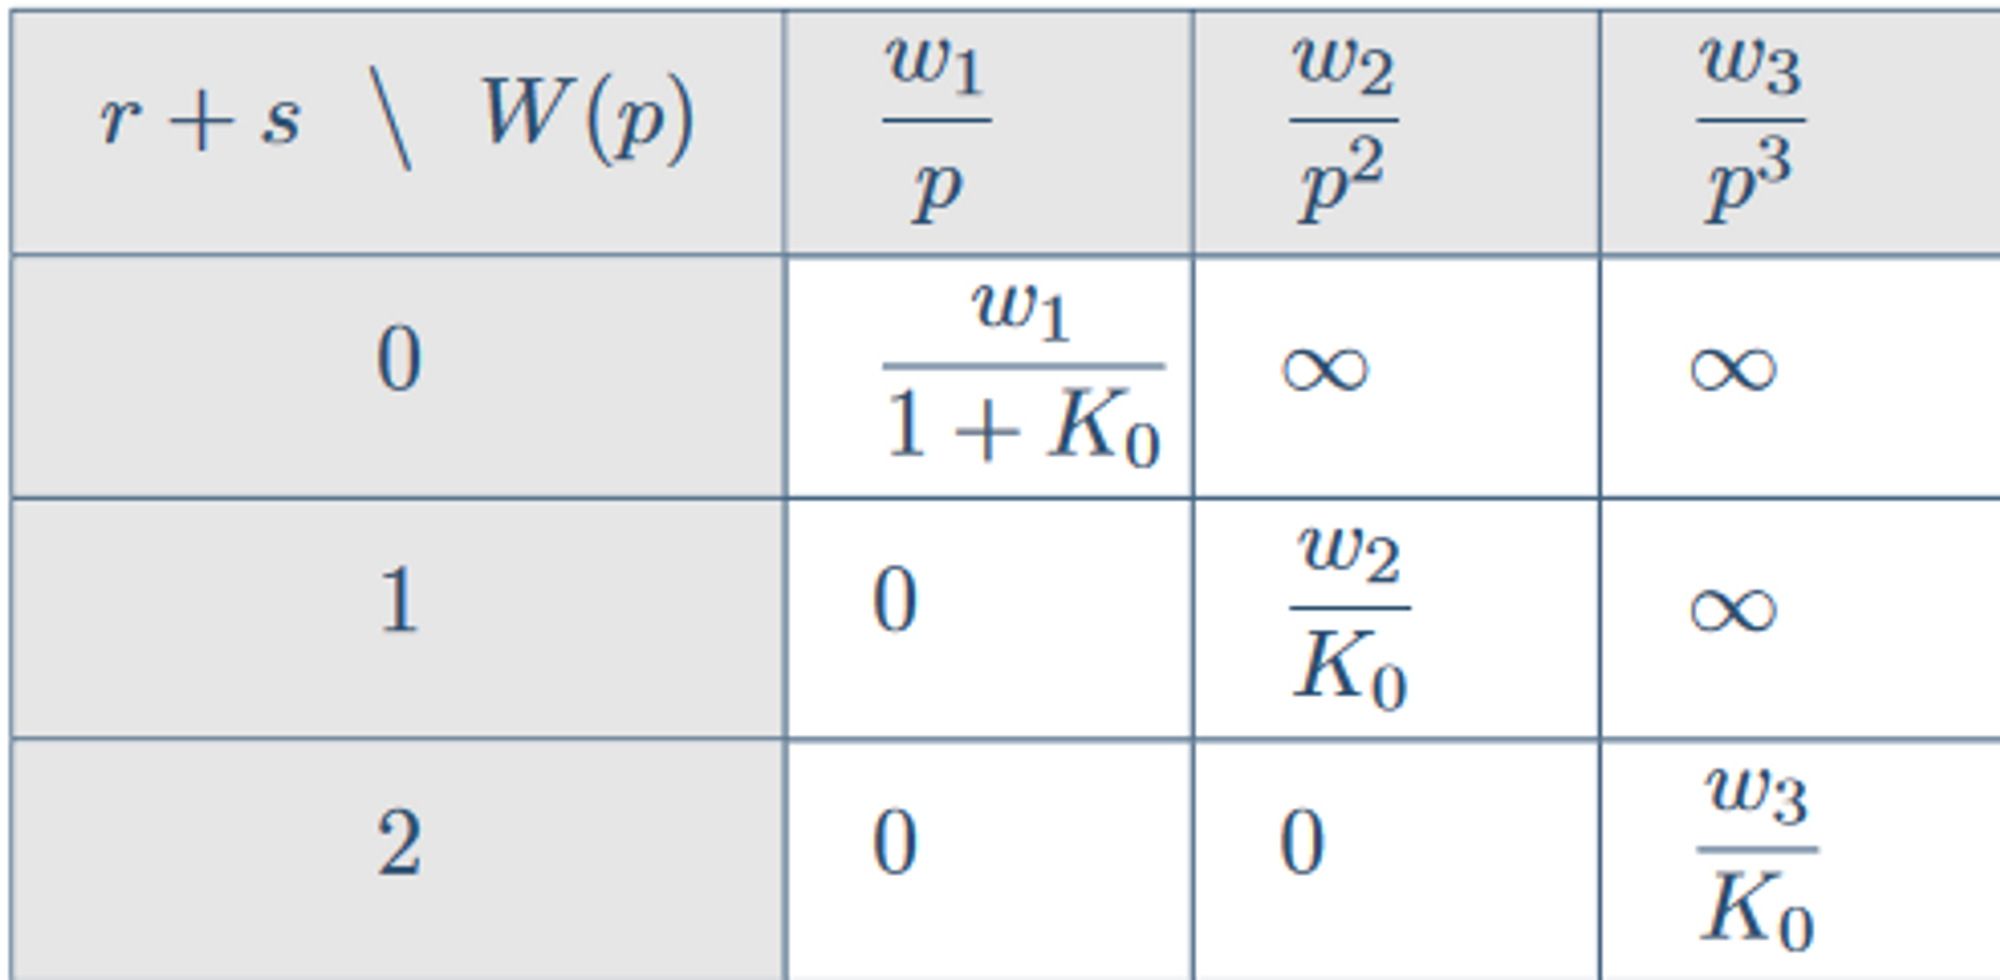
\includegraphics[scale = 0.3]{images/ustalena_odchylka.png}
\end{figure}
\newpage
Ustálená odchylka pro různý typy poruch a počet integrátorů v soustavě a vregulátoru:
\begin{figure}[H]
    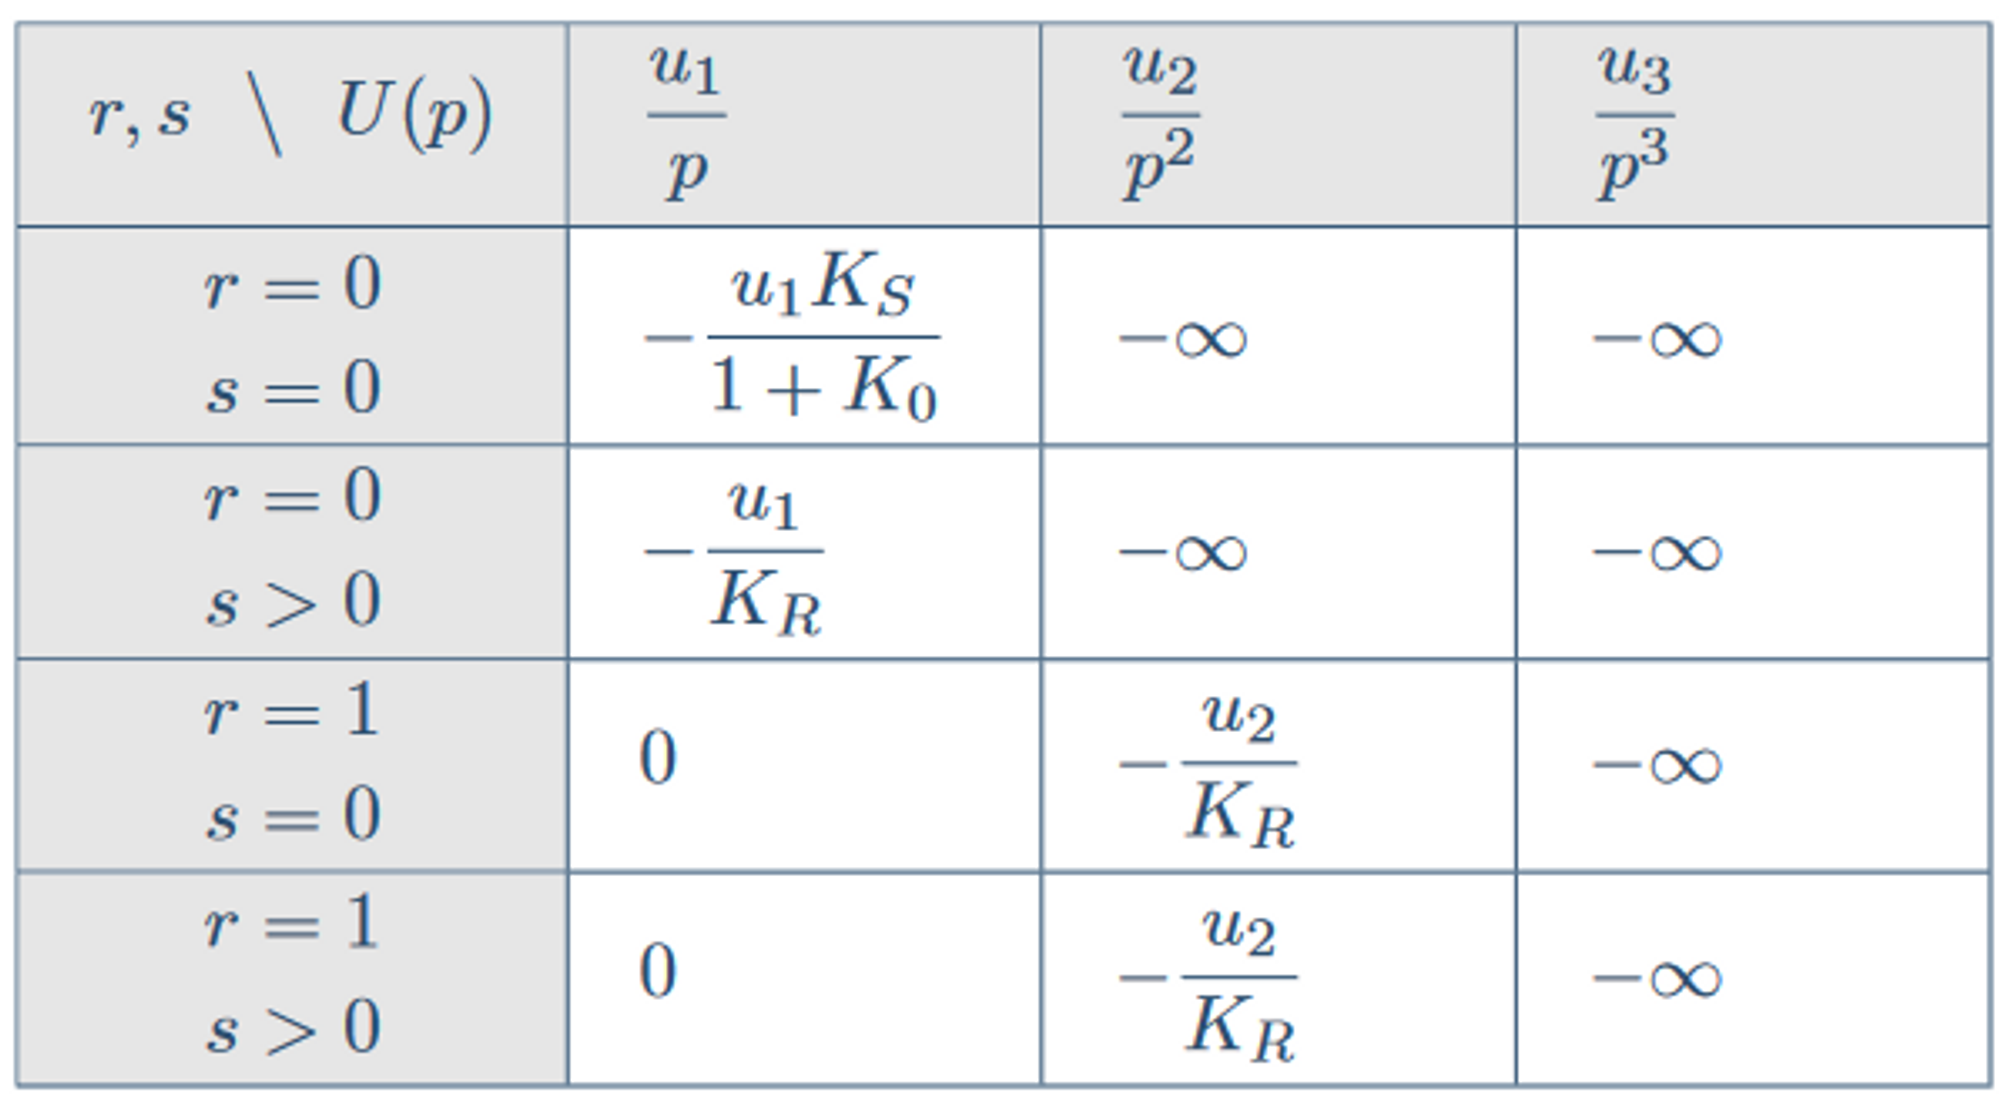
\includegraphics[scale = 0.3]{images/ustalena_odchylka2.png}
\end{figure}
\newpage

\section{Standardní struktury regulačních obvodů. Stabilita obvodů se zpětnou vazbou. Frekvenční charakteristiky v komplexní rovině, Nyquistovo kritérium stability, jeho zjednodušená verze a řešení v logaritmických souřadnicích, použití algebraických kritérií.}
PID:
\begin{figure}[H]
    \includegraphics*[scale = 1.1]{images/PIDschema.png}
\end{figure}


PSD:
\begin{figure}[H]
    \includegraphics*[scale = 1.1]{images/PSDschema.png}
\end{figure}
\newpage

Rozdělení podle stupňů volnosti(kolik regulátorů, tolik stupňů):
\begin{itemize}
    \item jeden stupeň volnosti - odchylkový regulátor
          \begin{figure}[H]
              \includegraphics*[scale = 0.45]{images/jedenStupenVolnostii.png}
          \end{figure}
    \item dva stupňě volnosti(lze plnit požadavky na změnu řízení i poruchy)
          \begin{figure}[H]
              \includegraphics*[scale = 0.4]{images/dvaStupenVolnostii.png}
          \end{figure}
\end{itemize}

\subsection*{Stabilita obvodů se zpětnou vazbou}
Lineární systém je stabilní, pokud výstup po skončení budícího signálu a doznění přechodného děje vrátí na původní hodnotu.\\
Další podmínkou je, když odezva na omezený budící signál je taky omezená, nebo přítomnost všech pólů přenosové funkce v levé polorovině komplexní roviny p(u diskrétních uvnitř jednotkové kružnice).\\

Je několik způsobů, jak určit stabilitu:
\begin{itemize}
    \item Stabilita z charakteristické rovnice
    \item Nyquistovo kritérium stability
    \item Zjednodušené Nyquistovo kritérium
\end{itemize}


\subsubsection*{Stabilita z charakteristické rovnice}
Aby byl zpětnovazební systém stabilní, musí kořeny charakteristické rovnice být v lévé polorovině komplexní roviny p.\\
V charakteristické rovnici se často nachází neznámé proměnné, jsou algebraická kritéria výhodnější(Hurwitz a Routh-Schur).\\

\subsubsection*{Nyquistovo kritérium stability}
Slouží k určení stability uzavřené smyčky.\\
Stabilita se rozhoduje na základě průběhu frekvenční charakteristiky otevřené smyčky a poloze jejich pólů.\\
Využívá se Cauchyho teorému o fázi - mapování uzavřené křivky z roviny p do roviny F.\\
\begin{equation}
    F(p) = \frac{B(p)}{A(p)} = k\frac{(p-\beta_1)(p-\beta_2)\dots (p-\beta_m)}{(p-\alpha_1)(p-\alpha_2)\dots (p-\alpha_m)}
\end{equation}
\begin{figure}[H]
    \includegraphics*[scale = 0.3]{images/NyQuistMapovani.png}
\end{figure}
\textbf{Jestliže uzavřená záporně orientovaná křivka v rovině p obkličuje b nul a a pólů přenosu F(p) a neprochází žádným jejím pólem ani nulou, potom uzavřená křivka vzniklá mapováním obíhá počátek roviny b - a krát v záporném směru}.\\
Pro odvození Cauchyho teorému je důležitá změna fáze uzavřené orientované křivky v rovině F. Fáze přenosu je dána součtem jednotlivých příspěvků kořenových činitelů čitatele $(p - \beta_i)$, od  kterých se odečte součet jednotlivých příspěvků kořenových činitelů jmenovatele $(p - \alpha_i)$.\\
\newpage

Vliv kořenů na změnu fáze uzavřené křivky:
\begin{figure}[H]
    \includegraphics*[scale = 0.3]{images/NyQuistVlivKorenu.png}
\end{figure}
Příspěvek pólů a nul uvnitř křivky je $2\pi$ s tím, že příspěvek pólů se bere se záporným znaménkem.\\
V tomto případě je příspěvek nulový, jelikož pól a nula se odečtou.\\
Využití Cauchyho teorému u Nyquistova kritéria stability:\\
\begin{itemize}
    \item Vytvoření záporně orientované křivky, která obkličuje celou pravou polorovinu roviny p
    \item Uzavřený systém bude stabilní, pokud bude frekvenční charakteristika pro $\omega = (-\infty, \infty)$ obíhat počátek roviny F v kladném směru tolikrát, kolik nestabilních pólů má přenos F(p)
    \item Jednodušší je sledovat počet oběhů funkce $F_0$ kolem bodu (-1,0)
\end{itemize}

Pro případ, kdy máme póly v počátku je nutné je zahrnout buď do pravé, nebo levé poloroviny(zpravidla se zahrnuje do levé, ale funguje na obě strany) - křivka bude pól obcházet s minimálním poloměrem.\\
To že jsme je zahrnuli např. do levé poloroviny neznamená, že jsou stabilní, pouze s nimi v rámci Nyquistova kritéria jako se stabilními počítáme.\\
\begin{figure}[H]
    \includegraphics*[scale = 0.15]{images/NyQuistPocatek.png}
\end{figure}

\subsubsection*{Zjednodušené Nyquistovo kritérium}
Pokud přenos otevřené smyčky neobsahuje póly v pravé polorovině komplexní roviny p, lze použít zjednodušené Nyquistovo kritérium stability.\\
\begin{figure}[H]
    \includegraphics*[scale = 0.4]{images/NyQuistZjednoduseny.png}
\end{figure}

Uzavřený systém je stabilní, jestli při frekvenci řezu je fáze kladnější, než $-\pi$.\\

\subsubsection*{Algebraické kritéria}
Nevýhodou algebraických kritérií je, že i pro jednoduché příklady vznikají dosti složité řešení.\\
Výhodou je, že dostaneme rozsahy parametrů, pro které je Uzavřený obvod stabilní.\\
Hurwitzuv determinant:
\begin{itemize}
    \item Z charakteristické rovnice se vytvoří čtvercová matice, ze které se určí determinant, který pro stabilitu musí být větší, než 0.
          \begin{figure}[H]
              \includegraphics*[scale = 1.2]{images/Hurwitz.png}
          \end{figure}
    \item Všechny podmínky vycházející z příkladu musí platit společně.
\end{itemize}


Routh-Schurovo kritérium:

\begin{itemize}
    \item všechny koeficienty v redukovaných řádcích musí mět stejné znaménko, aby byl systém stabilní
\end{itemize}
Vzorový příklad k charakteristickému polynomu: $0.1p^5+2.01p^4+10.2p^3+(K_0+1.0)p^2+2.0K_0p+K_0$
\begin{figure}[H]
    \includegraphics*[scale = 1.2]{images/RouthSchur.png}
\end{figure}
\begin{figure}[H]
    \includegraphics*[scale = 1]{images/RouthSchur2.png}
\end{figure}




\section{Analýza dymanických vlastností zpětnovazebních obvodů. Metoda geometrického místa kořenů. Zásoba stability v amplitudě, fázi, modulu. Integrální kritéria kvality regulace, praktická kritéria}
Dynamickými vlastnostmi popisujeme chování systému v přechodných dějích. Tím je myšleno rchlost odeznění, maximální překmit a kmitavost přechodného děje. Neexistuje univerzálně optimálně navrhnutý regulátor, dost záleží na situaci.
Dynamické vlastnosti se zjišťují z těchto hledisek:
\begin{itemize}
    \item z rozložení nul a pólů v komplexní rovině
    \item z odezev v časové oblasti
    \item z průběhu frekvenčních charakteristik
\end{itemize}


\subsection*{Metoda kořenového hodografu}
Jedná se o zobrazení průběhu pólů charakteristické rovnice v závislosti na proměnlivém parametru v komplexní rovině.\\
Postup grafického řešení:
\begin{itemize}
    \item v přenosu otevřené smyčky za p dosaíme \(p_0\) jako konkrétní bod
    \item dále vektor $(p_0 - \alpha_1)$ se dá zapsat v goniometrickém tvaru jako $|p_0 - \alpha_1|\angle (p_0 - \alpha_1)$
    \item fázi získáme tak, že součtem fáze v čitateli a odečtem fáze ze jmenovatele
    \item modul je dělení čitatele jmenovatelem
    \item vzorový příklad:
          \begin{figure}[H]
              \includegraphics*[scale = 0.3]{images/hodograf.png}
          \end{figure}
\end{itemize}

\subsubsection*{Soubor pravidel pro konstrukci kořenového hodografu}
\begin{itemize}
    \item Symetrie - kořenový hodograf je symetrický kolem reálné osy
    \item Počet větví - kořenový hodograf obsahuje n větví
    \item Segmenty na reálné ose - pokud napravo od části reálné osy leží lichý počet nul a pólů, tak tato část osy je větev kořenového hodografu
    \item Počátky a konce větví - každá větev začíná při zesílení K = 0 v pólu a končí v K = $\infty$ v nule. Pokud je v přenosu víc pólů, jak nul, tak n - m větví odchází do nekonečna podle přímkových asymptot
    \item Poloha asymptot - asymptoty se protínají na reálné ose v bodě $\sigma = \frac{\sum^n_{i=1} \alpha_i - \sum^m_{i=1}\beta_i}{n-m}$ a svírá s kladnou reálnou poloosou úhel $\varphi = \frac{180 \degree + i360\degree}{n - m}$ \dots i = 0, 1 ..., n-m-1
    \item Průsečík s imaginární osou - hodnota K, pro kterou prochází větve kořenového hodografu imaginární osou se dá určit pomocí algebraických kritérií stability
    \item Úhel v komplexní nule nebo pólu - úhel tečny, se kterým vychází větev kořenového hodografu z komplexního pólu $\alpha_k$ se vypočítá jako $\gamma_k = 180 \degree + i360 \degree -\sum^n_{i=1, i\neq k}\angle(\alpha_k - \alpha_i) + \sum^m_{i=1}\angle(\alpha_k - \beta_i)$. Úhel tečny, se kterým vchází větev kořenového hodografu do komplexní nuly $\beta_k$, se vypočítá jako $\delta_k = 180 \degree + i360 \degree -\sum^n_{i=1}\angle(\beta_k - \alpha_i) + \sum^m_{i=1, i\neq k}\angle(\beta_k - \beta_i)$
    \item Průsečík s reálnou osou - průsečík větve kořenového hodografu s reálnou osou se většinou analyticky vyřešit nedá, řeší se iterativně
\end{itemize}
\subsection*{Zásoba stability v amplitudě, ve fázi a v modulu}
\subsubsection*{Zásoba stability v amplitudě}
Hodnota zesílení, se kterou když vynásobíme stávající zesílení otevřené smyčky, tak přivedeme uzavřenou smyčku na mez stability.\\
Udává se ve formě násobícího faktoru nebo v decibelech.\\
Značí se Mg. Je to převrácená vzdálenost místa kde frekvenční charakretistika protíná zápornou reálnou osu a počátku soustavy souřadnic.\\

\subsubsection*{Zásoba stability ve fázi}
Záporně vzatá změna fáze otevřeného obvodu, která přivede uzavřený obvod na mez stability.\\
Značí se Mp. Úhel mezi zápornou částí reálné osy a přímkou mezi počátkem a průsečíkem frekvenční chrakteristiky s kružnicí se středem v počátku a poloměrem 1.\\

\subsubsection*{Zásoba stability v modulu}
Nejkratší vzdálenost frekvenční charakteristiky otevřené smyčky do bodu -1 v komplexní rovině.\\
Silnější kritérium než Mg a Mp.\\

\begin{figure}[H]
    \centering
    \includegraphics*[scale = 1.2]{images/zasobaStabiliity.png}
\end{figure}
\begin{figure}[H]
    \includegraphics*[scale = 1.1]{images/zasobaStabiliityTabulka.png}
\end{figure}


\subsection*{Integrální kritéria kvality regulace, praktická kritéria}
Výčet kritérií:
\begin{itemize}
    \item Lineární
    \item Usměrněné lineární
    \item Kvadratické
    \item ITAE
\end{itemize}
\newpage

\subsubsection*{Lineární}
Odečtení ustálené odchylky zajišťuje konvergenci integrálu k nějaké konečné hodnotě.\\
\begin{equation}
    J_L = \int^\infty_0[e(t) - e(\infty)]dt
\end{equation}
Počítá plochu mezi průběhem regulační odchylky e(t) a ustálenou odchylkou e(\(\infty\)).
Musí se dodržet, že celá odchylka se pohybuje v kladné hodnotě, jinak nemá smysl, proto se moc nepoužívá.\\
\begin{figure}[H]
    \includegraphics*[scale = 0.3]{images/linearniKriterium.png}
\end{figure}

\subsubsection*{Usměrněné lineární kritérium}
Dá se člen integrálu do absolutní hodnoty.\\
Problém nelinearita u středu.
\begin{equation}
    J_{UL} = \int^\infty_0|e(t) - e(\infty)|dt
\end{equation}
\begin{figure}[H]
    \includegraphics*[scale = 0.3]{images/usmerneneLinearniKriterium.png}
\end{figure}

\subsubsection*{Kvadratické kritérium}
Člen integrálu se dá na druhou.\\
Problém optimální průběhy jsou hodně kmitavé.\\
Přisuzuje se větší váha větším odchylkám. Z čehož plyne nevýhoda, protože na začátku je generován velký překmit kvůli rychlé kompenzaci velkých odchylek.\\
\begin{equation}
    J_K = \int^\infty_0[e(t) - e(\infty)]^2dt
\end{equation}
\begin{figure}[H]
    \includegraphics*[scale = 0.3]{images/kvadratickeKriterium.png}
\end{figure}
Druhy výpočtu:
\begin{itemize}
    \item Výpočet \(\mathfrak{L}^{-1}\{E(o)\}\) s integrací podle \(J_K = \int^\infty_0[e(t) - e(\infty)]^2dt\)
    \item Analytický výpočet pomocí reziduové věty
    \item Pomocí Nekolného doplňku k Routh-Schurově algoritmu
    \item Pomocí simulace
\end{itemize}
Existuje analytické řešení - Nekolného doplněk:
\begin{figure}[H]
    \includegraphics*[scale = 1]{images/nekolnehoDoplnek.png}
\end{figure}

\subsubsection*{ITAE kritérium}
Nejpoužívanější\\
Nedá se řešit analyticky.\\
\begin{figure}[H]
    \includegraphics*[scale = 0.3]{images/ITAE.png}
\end{figure}
Zhodnocení vlastností:
\begin{itemize}
    \item méně kmitavý průběh ve srovnání s kvadratickým
    \item váhové kritérium - váha odchylky narůstá s časem
    \item analytický výpočet prakticky nemožný, řešení simulace
\end{itemize}
\newpage


\section{ Návrh PID regulátorů různými metodami (metoda standardních tvarů frekvenčních charakteristik, metoda optimálního
  modulu, metoda Zieglera-Nicholse, metoda standardních tvarů charakteristického polynomu, metoda požadovaného
  rozložení pólů uzavřeného obvodu).}

\subsection*{Metoda standartních tvarů frekvenčních charakteristik}

Tvarujem frekveční charakteristiku tak, abychom dosáhli vyhovujícího tvaru - obecně platný postup neexistuje.\\
Průběh soustavy i regulátoru se sčítají za předpokladu, že jsou charakteristiky v decibelech.\\
Obecné požadavky na přenos:
\begin{itemize}
    \item co nejvyšší hodnota kmitočtu řezu - rychlost děje
    \item co největší fázová bezpečnost - zajišťuje malý překmit(co nejvíc kladná oproti -180°)
    \item kolem kmitočtu řezu v co největším okolí sklon -20dB/dek
    \item Realizovatelnost - řád jmenovatele větší než řád čitatele regulátoru (PID a PD se dává realizační konstanta do jmenovatele, obvykle se volí tak, že časová konstanta čitatele je míň jak 100x větší )
\end{itemize}
Hodnota řezu je místo kde frekvenční charakteristika nabývá hodnoty 0dB.
\begin{figure}[H]
    \includegraphics*[scale = 0.8]{images/freqNavrh.png}
\end{figure}
\newpage

\subsection*{Metoda optimálního modulu}
Oproti návrhu z frekvenční charakteristiky pracuje tato metoda s frekvenční charakteristikou uzavřené smyčky(FW). $F_W(p) = \frac{b_mp^m+b_{m-1}p^{m-1}+\dots + b_1p+b_0}{a_np^n+a_{n-1}p^{n-1}+\dots + a_1p+a_0}$\\
Založená na tom, že přechodný děj bude optimální. pokud FW $\doteq$ 1 do co nejvyšších frekvencí.\\
To se dá zapsat matematicky jako: $\frac{d|F_W(j\omega) |}{d\omega} \leq 0$\\
Postup:
\begin{enumerate}
    \item p se nahradí $j\omega$
    \item čitatel i jmenovatel se vyjádří ve tvaru reálná složka + imaginární složka
    \item spočítá se absolutní hodnota přenosu (tj. každý člen na druhou a celé pod odmocninou)
    \item stejné podmínky platí i pro druhou mocninu přenosu, tak se dá nadruhou, aby se nemuselo počítat s odmocninou
          \begin{figure}[H]
              \includegraphics*[scale = 1.0]{images/optimalniModul1.png}
          \end{figure}
    \item porovnáním rovnic dostaneme toto:
          \begin{figure}[H]
              \includegraphics*[scale = 1.0]{images/optimalniModul2.png}
          \end{figure}
    \item Dříve uvedné podmínky pro optimální průběh lze vyjádřiit ve formě
          \begin{equation}
              \frac{B_i}{A_i} \leq \frac{B_0}{A_0}
          \end{equation}
\end{enumerate}

Tímto je zaručena monotónost průběhu, ale NEZARUČUJE STABILITU OBVODU.  Nutné zvlášť dopočítat.
(Vzorový příklad viz skripta, nebo coz rr1)\\
\newpage

\subsection*{Metoda Zieglera-Nicholse}
V praxi oblíbená a hojně používaná.\\
Vychází se z PID regulátoru ve tvaru: $F_R(p) = K_R(1+\frac{1}{T_Ip}+T_Dp)$
Princip:
\begin{enumerate}
    \item Vyřadíme integrační a derivační složku($T_D = 0$ a $T_I = \infty$)
    \item Zvyšujeme zesílení proporciální složky $K_R$, dokud nedosáhneme meze stability. Čímž dosáhneme netlumených kmitů a taky hodnoty $K_{KRIT}$ a $T_{KRIT}$
    \item Hodnoty jednotlivých složek určíme z tabulky
          \begin{figure}[H]
              \includegraphics*[scale = 1]{images/ZHtab.png}
          \end{figure}
\end{enumerate}
Kriitické parametry se dají určit několia způsoby:
\begin{itemize}
    \item Z přechodové charakteristiky
    \item výpočtem ze známého modelu
    \item rozkmitávání použitím relé bez hysterze
\end{itemize}

\subsubsection*{Určení kritických parametrů z přechodové charakteristiky}
Odečtením doby průtahu $T_u$ a doby náběhu $T_n$ a následně dopočítat pomocí vzorců:
\begin{equation}
    K_{KRIT} \doteq \frac{\pi T_n}{2T_u}+1 \;\;\;\;\;\;\;\;\;\;\;\;\;\;\;\;\;\; T_{KRIT} \doteq 4T_u
\end{equation}

\subsubsection*{Určení kritiiických parametrů výpočtem ze známého modelu}
Existuje několik způsobů, jeden z nich je pomocí Nyquistova kritéria stability. Uzavřený obvod je na mezi stability pokud frekvenční charakteristika otevřené smyčky prochází bodem (-1;0). Následně se určí průsečík frekvenční charakteristiky otevřené smyčky se zápornou částí reálné osy(-x;0). Kritické zesílení je následně určeno jako $\frac{1}{x}$.\\
Pro soustavy vyššího řádu je obtížné najít průsečík, proto se využívá algebraických kritérií stability(Hurwitzh nebo Routh-Schur)

\subsubsection*{Rozkmitávání použitím relé bez hysterze}
Velká výhoda, že kmity jsou řízené - nehrozí, že by se systém nekontrolovaně rozkmital.\\
Určuje se tak, že zvětšujeme zesílení, dokud relé  nezačne kmitat.\\

Metoda Ziegler-Nicholse je výhodná v případě, kdy nemáme k dispozici přenos soustavy a můžeme experimentovat. To občas může být nebezpečné, proto se pak využívá relé bez hysterze, kde se jedná o řízené kmitání.\\

\subsection*{Metoda standartních tvarů}
Vychazí se z toho, že kořeny charakteristiického polynomu určují dynamiku uzavřeného obvodu.\\
Koeficienty se určují z Whiteleyho tvarů, které se nachází v tabulce, jedná se o poměry jednotlivých složek. Platí pouze pro soustavy s astatismem prvního řádu.\\
\begin{figure}[H]
    \centering
    \includegraphics*[scale = 0.8]{images/metodaStandartnichTvaru.png}
\end{figure}
Pro použití tabulky je však nutné charakteristický polynom upravit na bezrozměrný tvar.\\
Regulátory navržené touto metodou mají malé zesílení a tím pádem tlumené a pomalé odezvy.\\
V tomto tvaru je první a poslední koeficient roven jedné.To se dělá pomocí koeficientu q, který se získá pomocí vzorce:
\begin{equation}
    \frac{a_n}{a_0}p^n = q^n
\end{equation}
Příklad:\\
\begin{center}
    Soustava: \(F_S(p)=\frac{0,1}{p(3p+1)(0,8p+1)}\) Regulátor PD: \(F_R(p)=K_R(Tp+1)\)\\
    Otevřená smyčka: \(F_0(p) = \frac{0,1K_R(Tp+1)}{p(3p+1)(0,8p+1)}\)\\
    Charakteristický polynom: \(2,4p^3+3,8p^2+(1+K_0T)p+K_0\)\\
    Normalizace koeficientu: \(\frac{2,4}{K_0}p^3+\frac{3,8}{K_0}p^2+\frac{1+K_0T}{K_0}p+\frac{K_0}{K_0}\)\\
    Substituce: \(\frac{2,4}{K_0}p^3 = q^3 \rightarrow q = q \sqrt[3]{\frac{K_0}{2,4}} \)\\
    Pak tedy: \(q^3 + \frac{3,8}{K_0}(\frac{K_0}{2,4})^{\frac{2}{3}}q^2+\frac{1+K_0}{K_0}\sqrt[3]{\frac{K_0}{2,4}}q+1\)\\
    Máme regulátor PD a stupeň polynomu 3, podle toho vybereme z tabulky:\\
    \(\frac{3,8}{K_0}(\frac{K_0}{2,4})^{\frac{2}{3}} = 5,1\) a \(\frac{1+K_0}{K_0}\sqrt[3]{\frac{K_0}{2,4}} = 6,3\) z toho vyjde \(K_0 = 0,072\)\\
    Pak máme: \(K_R = \frac{F_0}{0,1} = 0,72\) a \(T = 6,36\)\\
    PD regulátor: \(F_R(p) = 0,72(6,36p+1)\)
\end{center}

\subsection*{Metoda požadovaného rozložení pólů uzavřeného obvodu}
Tato metoda využívá vztahu mezi časovými odedzvami a rozložením pólů v přenosu uzavřené smyčky. Využívá se konstrukce kořenového hodografu.\\
Stanovíme si požadavky na tlumení obvodu a tím vymezíme jistou oblast v rovině p, ve které mohou ležet póly.
Čím větší tlumení zvolíme, tím menší úhel bude svírat reálná osa s výsečí. Větší roli hrají dominantní póly(ty blíže ke středu) a zrychlení odezvy dosáhneme posunem těchto pólů co nejvíc vlevo(viz d)\\
\begin{figure}[H]
    \includegraphics*[scale = 1]{images/metodaRozlozeniPolu.png}
\end{figure}


\newpage


\section{PSD regulátory, základní složky a vlastnosti. Aproximace vzorkovače s tvarovačem, diskretizace PID regulátoru.
  Rozvětvené regulační obvody. Obvod s pomocnou regulovanou veličinou, s pomocnou akční veličinou, s měřením
  poruchy, s modelem regulované soustavy (kompenzace dopravního zpoždění). Vícerozměrové řídicí systémy.}

Popis stejný jak spojitý PID akorát v diskrétní oblasti.\\
Převod mezi spojitým a diskrétním přenosem se dělá pomocí Z-transformace. Dochazí zde ke zpoždění o 0,5 vzorkovací periody.
\begin{figure}[H]
    \includegraphics*[scale = 1]{images/PSDVzorkovani.png}
\end{figure}
Integrační složka se nahrazuje sumou: \(\int_{0}^{t}e(\tau)d\tau = \int_{0}^{NT}e(\tau)d\tau \rightarrow T_{vz}\sum_{n = 0}^{N}e(n) \approx \frac{T_{vz}}{1-z ^{-1}} \)\\
Derivační složka se nahrazuje výpočtem diference: $\frac{de}{dt} \rightarrow \frac{e(k)-e(k-1)}{t_{vz}} = \frac{1-z^{-1}}{T_{vz}}$.\\
Tvary PSD regulátoru:
\begin{itemize}
    \item $F_R(z^{-1}) = K_R(1+\frac{T_D}{T_{vz}}(1-z^{-1})+\frac{T_{vz}}{T_I}\frac{1}{1-z^{-1}})$
    \item $u(k) = K_R(e(k)+\frac{T_D}{T_{vz}}(e(k)-e(k-1))+\frac{T_{vz}}{T_I}\sum^k_{i=1}e(i))$
\end{itemize}
\begin{figure}[H]
    \centering
    \includegraphics*[scale = 0.3]{images/PSD_regulator.png}
\end{figure}
\newpage

Z důvodu vzorkování se počítá, že přechodová charakretistika je zpožděná o polovinu vzorkovací periody:
\begin{figure}[H]
    \centering
    \includegraphics*[scale = 0.27]{images/PSDVzorkovaniZpozdeni.png}
\end{figure}

\subsubsection*{Konečná doba přechodného děje}
Existují dva případy:
\begin{itemize}
    \item v okamžicích vzorkování
    \item i mezi okamžiky vzorkování
\end{itemize}
V okamžicích vzorkování je podmínka, aby dva po sobě jdoucí vzorky byly nulové.\\
V druhém případě musí vyhovovat i diference hodnot y[(m + n)t] a y[(m + 1 + n)t], kde $0 \leq m \leq 1$\\
Vychází se z rovnice přenosu $F_W(z) = f_0 + f_1z^{-1}+f_2z^{-2} \dots $ \\
Přechodný děj je konečný i v časech mimo vzorkování, jestli že F(z,m) má konečný počet členů pro všechna m z intervalu <0;1>. To je splněno pouze, když funkce FW(z,m) obsahuje celý čitatelový polynom přenosu spojitě pracující části obvodu P(z,m).\\
\subsubsection*{Aproximace vzorkovače s tvarovačem}
Tvarovač nultého řádu.Dopředný(generuje se zpětně), zpětný(klasická vzorkovačka nultého řádu), aproximační(spojuje dvě hodnoty vzorkovací - aproximace 1.řádu)
\begin{figure}[H]
    \includegraphics*[scale = 1]{images/tvarovace.png}
\end{figure}

\subsection*{Rozvětvené regulační obvody}
Jsou-li na kvalitu regulace kladeny vyšší nároky, využívá se rozvětvených regulačních obvodů.
Hlavní typy jsou:
\begin{itemize}
    \item s pomocnou regulovanou veličinou
    \item s pomocnou akční veličinou
    \item s měřením poruchy
    \item s modelem regulované soustavy
\end{itemize}

\subsection*{Obvody s pomocnou regulovanou veličinou}
V tomto případě je místo bloku soustavy regulovaná soustava(S1+R2) v sérii s S2 a hlavní regulátor je R1. Často se využívá k regulaci teploty a v polohových servomechanismech. Při regulaci teploty je soustava tvořena větším počtem setrvačných článků spojených sériově. Zavedením pomocné regulované veličiny u vstupu do soustavy jsme schopni rychleji reagovat na vznik poruchy. \\
Pěkné příklady jsou ve skriptech rr1 str.154.
\begin{figure}[H]
    \includegraphics*[scale = 1]{images/pomocnaRegulace.png}
\end{figure}
Pomocí Z-N metody se dá dosáhnout automatizace opakovaným navrhováním(info navíc asi).\\

\subsection*{Regulační obvody s pomocnou akční veličinou}
Podmínkou pro realizaci je možnost působit na soustavu nejméně dvěmi akčními veličinami. Musí se lišit velikost časových konstant obou přenosů a to z důvodu, že akční zásah jedné akční veličiny musí být rychleji přenášen na soustavu, než změna druhé akční veličiny. Pomocnou akční veličinou výrazně zlepšíme přenos řízení.\\
Pěkné příklady rr1 skripta str.157.
\begin{figure}[H]
    \includegraphics*[scale = 1]{images/pomocnaAkcniVelicina.png}
\end{figure}

\subsection*{Regulační obvody s měřením poruchy}
Teoreticky lze pomocí regulátoru R2 dosáhnout úplné kompenzace poruchy(invariantnosti systému vůči poruše). U reálného regulátoru je to však omezeno podmínkou, kdy přenos poruchy musí být vyššího nebo stejného řádu jak přenos soustavy, což málokdy nastává. Na stabilitu systému pomocný regulátor R2 nemá vliv.\\
Bývá realizováno při regulaci velkého objemu teplot(vytápění budov).
\begin{figure}[H]
    \includegraphics*[scale = 1]{images/pomocnaPorucha.png}
\end{figure}

\subsection*{Regulační obvody s modelem regulované soustavy}
Primárně se používají v adaptivních obvodech, ale dají se použít pro zlepšení vlastností i v jednoduchém regulačním obvodu.\\
Hlavní přínos je necitlivost kvality regulace na změnu parametrů soustavy, to zajišťuje regulátor M, který vyrovnává rozdíly mezi soustavou a jejím modelem.
\begin{figure}[H]
    \includegraphics*[scale = 1]{images/pomocnaModelRegulovaneSoustavy.png}
\end{figure}
\newpage

Speciálním případem je obvod kompenzující přítomnost dopravního zpoždění. Dle schématu soustava obsahuje dopravní zpoždění o velikosti $\Delta$.
\begin{figure}[H]
    \includegraphics*[scale = 1]{images/pomocneDP.png}
\end{figure}
V charakteristickém polynomu se nevyskytuje člen s dopravním zpoždění, což přispívá ke stabilitě systému. Realizace modelu ve spojité variantě by byla náročná a nákladná, proto se v praxi používá její diskrétní model.
\subsection*{Vícerozměrové řídící systémy}
Většina regulovaných soustav má více vstupů a více výstupů, s čímž se váže víc akčních veličin, poruch atd. Jelikož závisí na pořadí nasobení jednotlivých matic, pravidla blokové algebry jsou modifikovány.\\
I když počet vstupů a výstupů se většinou liší, bývají doplněny nulovými a to z důvodu, že práce se čtvercovými maticemi jsou jednodušší.
\begin{figure}[H]
    \includegraphics*[scale = 1]{images/vicerozmerneSoustavy.png}
\end{figure}
Vztah je popsán maticově, vyplývá z něj, že každý vstup ovlivňuje každý výstup.
\begin{equation}
    Y(p) = S(p)\cdot X(p)
\end{equation}
Jedním z hlavních požadavků na Vícerozměrné systémy je autonomnost. Systém je autonomní, pokud změna k-té žádané hodnoty způsobí změnu k-té regulované veličiny a na ostatních se neprojeví. Což by nastalo, kdyby matice soustavy byla diagonální, pokud tomu tak není, je nutné nežádoucí vazby mezi sobě neodpovídajícími akčními a regulovanými veličinami kompenzovat vhodnými vazbami v regulátorech. Proto každá akční veličina může být vázána na jakoukoliv regulační odchylku.\\
\begin{figure}[H]
    \includegraphics*[scale = 1]{images/vicerozmerneSoustavySchema.png}
\end{figure}
Ve většině systémů nejde dosáhnout úplné autonomnosti, proto se často spokojíme i s autonomností ustálených stavů, neboli že přenos je diagonální.\\
Další požadavek je invariantnost, což je necitlivost vůči poruchám. Úplné invariantnosti lze dosáhnout pouze, když je informace k poruchách, neboli poruchy lze měřit.
diagonální matice přenosů:

\begin{figure}[H]
    \includegraphics*[scale = 1]{images/DiagonalniMaticePrenosu.png}
\end{figure}


